\item \textbf{{[}NYJC/PRELIM/9569/2020/P1/Q2{]} }

In Morse code, each letter of the alphabet is represented by a unique
combination of dots and dashes. Study the following table carefully:
\noindent \begin{center}
\begin{tabular}{|c|c|c|}
\hline 
\textbf{Letter} & \textbf{Morse Code} & \tabularnewline
\hline 
\hline 
A & \texttt{. -} & dot dash\tabularnewline
\hline 
B & \texttt{- . . .} & dash dot dot dot\tabularnewline
\hline 
C & \texttt{- . - .} & dash dot dash dot\tabularnewline
\hline 
D & \texttt{- . . .} & dash dot dot\tabularnewline
\hline 
\end{tabular}
\par\end{center}

A binary tree is used to represent this coding system. Each node,
except the root node, contains a letter of the alphabet. The position
of each letter in the tree is determined by its Morse code. Moving
from one node to another down the tree is done by traversing either
a left branch or a right branch. A left branch corresponds to a .
(dot) and a right branch corresponds to a -- (dash). 

The first three levels of the tree are shown below:
\begin{center}
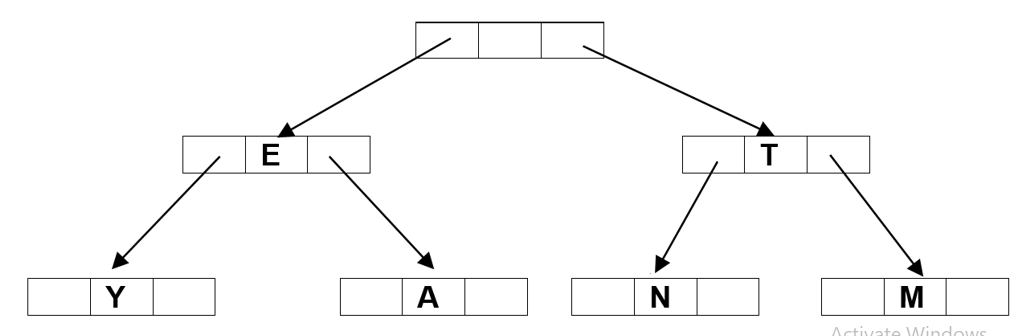
\includegraphics[width=0.5\paperwidth]{C:/Users/Admin/Desktop/Github/question_bank/LyX/static/img/9569-NYJC-2020-P1-Q2}
\par\end{center}
\begin{enumerate}
\item What are the Morse codes for the letters N and Y? \hfill{}{[}2{]}
\item Draw a diagram of the binary tree which clearly shows the position
of the letters D, C and B in the tree.\hfill{} {[}3{]}
\item {}
\begin{enumerate}
\item Explain why this binary tree representation is not the most suitable
data structure for performing English to Morse code conversion. \hfill{}{[}2{]}
\item Describe a better alternative and explain how the Morse code of a
letter could be found. \hfill{}{[}3{]}
\end{enumerate}
\end{enumerate}